\documentclass[12pt, twoside]{article}
\usepackage[letterpaper, margin=1in, headsep=0.5in]{geometry}
\usepackage[english]{babel}
\usepackage[utf8]{inputenc}
\usepackage{amsmath}
\usepackage{amsfonts}
\usepackage{amssymb}
\usepackage{tikz}
\usepackage{yhmath}
\usetikzlibrary{quotes, angles}
\usepackage{graphicx}
\usepackage{enumitem}
\usepackage{multicol}

\newif\ifmeta
\metatrue %print standards and topics tags

\title{Regents Geometry}
\author{Chris Huson}
\date{May 2022}

\usepackage{fancyhdr}
\pagestyle{fancy}
\fancyhf{}
\renewcommand{\headrulewidth}{0pt} % disable the underline of the header
\raggedbottom

\fancyhead[LE]{\thepage}
\fancyhead[RO]{\thepage \\ Name: \hspace{4cm} \,\\}
\fancyhead[LO]{BECA / Dr. Huson, Mr. Segal / Geometry\\* Unit 6: IB Geometry\\* 31 May 2022}

\begin{document}

\subsubsection*{6.14 Retest (optional) \hfill HSG.SRT.D.11}

\begin{enumerate}
  \item Right triangle $\triangle ABC$ is shown with side lengths marked.
  \begin{multicols}{2}
    \begin{enumerate}
      \item Which length is the hypotenuse? \vspace{0.5cm}
      \item Which length is \emph{opposite} angle $A$?  \vspace{0.5cm}
      \item Which length is \emph{adjacent} to angle $A$? %\vspace{0.25cm}
      \item What is the area of the triangle? \vspace{1cm}
      \item What fraction describes $\cos A$? \vspace{1cm}
    \end{enumerate}
  \begin{flushright}
          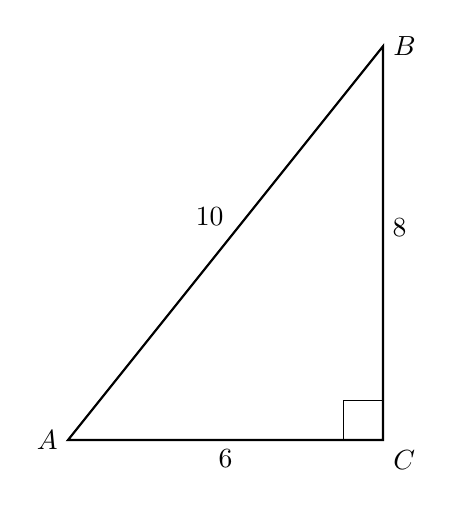
\begin{tikzpicture}[scale=1]
          \draw [thick]
          (0,0)node[left]{$A$}--
          (4,0)node[below right]{$C$}--
          (4,5)node[right]{$B$}--cycle;
          \draw (4,0)++(-0.5,0)--++(0,0.5)--+(0.5,0);
          \node at (2,0)[below]{$6$};
          \node at (4,2.7)[right]{$8$};
          \node at (1.8,2.6)[above]{$10$};
          %\node at (.25,.25) [right]{$\theta$};
          %\draw [thick, -] (1,0) arc [start angle=0, end angle=45, radius=1.2];
        \end{tikzpicture}
  \end{flushright}
  \end{multicols}
  
  \item Right triangle $\triangle PQR$ is shown with side lengths marked.
  \begin{multicols}{2}
    \begin{enumerate}[itemsep=0.4cm]
      \item Calculate the length PR.
      \item What fraction is $\sin \theta$?
      \item What fraction is $\cos \theta$?
      \item What fraction is $\tan \theta$?
      \item Which function of $\theta$ is $\displaystyle \frac{4}{8}$? \\($\tan$, $\sin$, or $\cos$)
      \item Find the area of the triangle.
    \end{enumerate}
  \begin{flushright}
          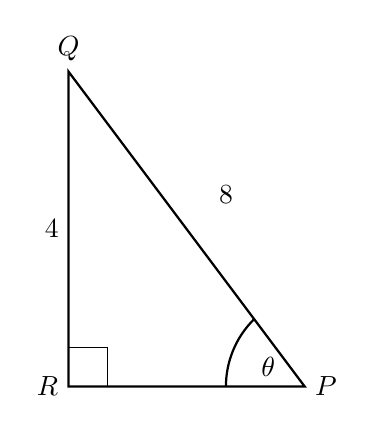
\begin{tikzpicture}[scale=1]
          \draw [thick]
          (2,0)node[right]{$P$}--
          (-1,4)node[above]{$Q$}--
          (-1,0)node[left]{$R$}--cycle;
          \draw (-.5,0)--++(-0,.5)--++(-.5,0);
          %\node at (2,0)[below]{$6$};
          \node at (-1,2)[left]{$4$};
          \node at (1,2.2)[above]{$8$};
          \node at (1.75,.25) [left]{$\theta$};
          \draw [thick, -] (1,0) arc [start angle=180, end angle=135, radius=1.2];
        \end{tikzpicture}
  \end{flushright}
  \end{multicols}
  \vspace{1cm}
  
  \item Find the area of the given triangle.
  \begin{flushright}
    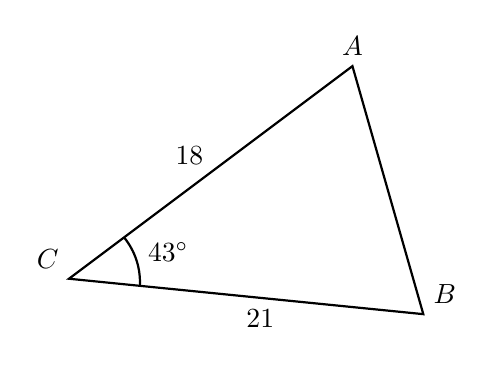
\begin{tikzpicture}[scale=0.9]
      \draw [thick]
        (0,0)node[above left]{$C$}--
        (5,-0.5)node[above right]{$B$}--
        (4,3)node[above]{$A$}--cycle;
     \draw [thick, -] (1,-0.1) arc [start angle=-3, end angle=39, radius=1];
     \node at (1.4,0.1)[above]{$43^\circ$};
     \node at (1.7,2)[below]{$18$};
     \node at (2.7,-0.3)[below]{$21$};
    \end{tikzpicture}
  \end{flushright}
  
  \newpage
  \item The following diagram shows triangle $PQR$, with $P\hat{Q}R=60^\circ$, $P\hat{R}Q=25^\circ$, and $PR=11$. \\[0.25cm]
  Find $PQ$. \hfill \emph{diagram not to scale}
    \begin{flushright}
      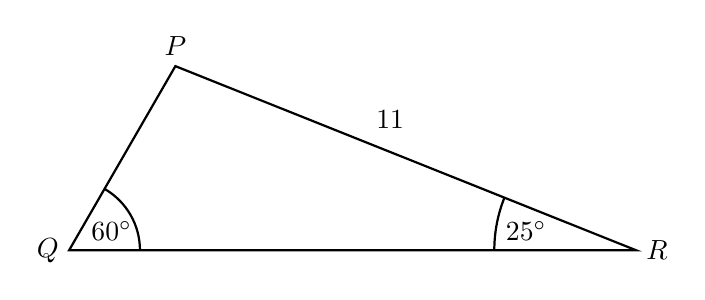
\begin{tikzpicture}[scale=.9]
        \draw [thick](60:3)node[above]{$P$}--
        (0,0)node[left]{$Q$}--
        (0:8)node[right]{$R$}--cycle;
        \node at (25:5)[below]{$11$};
        \draw [thick, -] (0:1) arc [start angle=0, end angle=60, radius=1];
        \node at (0:0.6)[above]{$60^\circ$};
        \draw [thick, -] (0:6) arc [start angle=180, end angle=158, radius=2];
        \node at (0:6.45)[above]{$25^\circ$};
      \end{tikzpicture}
    \end{flushright}\vspace{1cm}
  
  
  \item The following diagram shows triangle $DEF$, with $DE=7$, $D\hat{E}F=53^\circ$, and $EF=11$.  .\hfill \emph{diagram not to scale}
  \begin{multicols}{2}
  \begin{enumerate} [itemsep=1cm]
      \item Find ${DF}$. \vspace{1cm}
      \item What is the area of the triangle?
      \end{enumerate}
    \begin{flushright}
      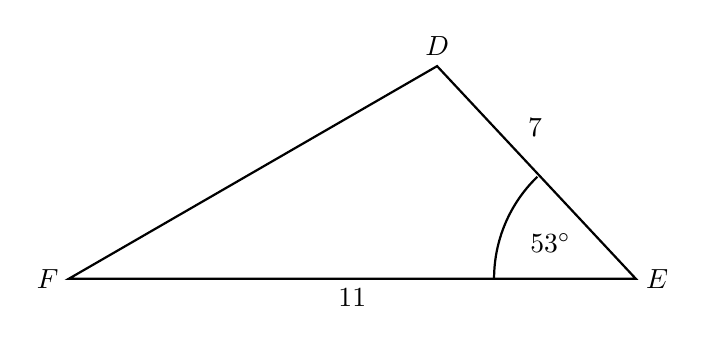
\begin{tikzpicture}[scale=.9]
        \draw [thick](30:6)node[above]{$D$}--
        (0,0)node[left]{$F$}--
        (0:8)node[right]{$E$}--cycle;
        \node at (20:7)[below]{$7$};
        %\draw [thick, -] (0:1) arc [start angle=0, end angle=60, radius=1];
        \node at (0:4)[below]{$11$};
        \draw [thick, -] (0:6) arc [start angle=180, end angle=134, radius=2];
        \node at (2:6.8)[above]{$53^\circ$};
      \end{tikzpicture}
    \end{flushright}
    \end{multicols} \vspace{2cm}
  
  \item Triangle $ABC$ has side lengths $AB=13.2$ and $AC=8.6$, while $A\hat{B}C=30^\circ$.
  \begin{flushright}
    \emph{diagram not to scale}
  \end{flushright}
  \begin{multicols}{2}
  \begin{enumerate}[itemsep=0.5cm]
      \item Find ${\sin C}$.
      \item Find $\angle C$.
      \end{enumerate}
    \begin{flushright}
      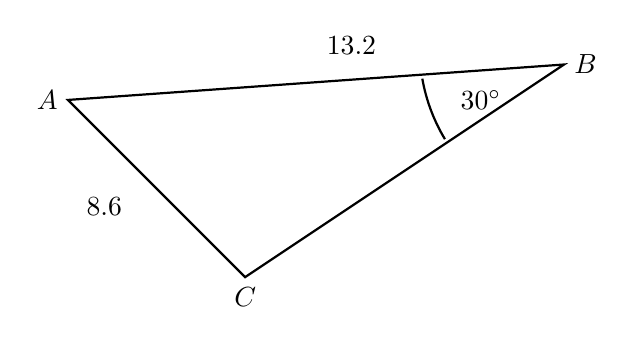
\begin{tikzpicture}[scale=0.9]
        %\draw [thick] (0,0) circle [radius=4];
        \draw [thick](-.5,0)node[below]{$C$}--
        (-3,2.5)node[left]{$A$}--
        (4,3)node[right]{$B$}--cycle;
        \node at (1,3)[above]{13.2};
        \node at (-2.1,1)[left]{8.6};
        \draw [thick, -] (2,2.8) arc [start angle=190, end angle=211, radius=2.5];
        \node at (3.25,2.5)[left]{$30^\circ$};
        %\node at (50:5.5)[above]{\emph{diagram not to scale}};
      \end{tikzpicture}
    \end{flushright}
  \end{multicols}
  

\end{enumerate}
\end{document}
  